\section{Introduction}
    
    As the size and complexity of engineering systems grow, the time and expense for setting up 
    analysis models grow with them. Multidisciplinary Design Analysis and Optimization (MDAO)
    frameworks such as OpenMDAO\cite{Gray2012} and ModelCenter have enabled a new level of analysis tool integration 
    and paved the way for models with more analyses and increasing numbers of interdisciplinary couplings. That 
    new capability has created a new challenge since configuring a model with the larger nubmer of analyses, associated inputs and outputs
    can be very difficult. Even for models with 10's of analyses, there could be hundreds of variables that need to be managed. 
    It is not hard to imagine that the task of combining all the analyses into a consistent system model capable of solving a relevant 
    engineering design problem could easily become much more costly than createing the discipline analyses themselves. Thus, for a large system
    as the couplings between the disciplines begin to dominate the design space, the couplings between the analyses begin to dominate 
    the job of setting up the model. 
    
    When building a model, coupling represents the reciprical flow of information between two analyses. 
    We propose the use of graph-based syntax to describe the flow of information from inputs, 
    through analyses, to outputs. If you allow for any free inputs to become design
    variables and some set of the outputs to become design objectives and constraints, then the graph 
    represents the problem formulation for a given design effort. 
    The graph-based syntax presented has application in all phases of the design process. 
    It can be used early on, to help construct a valid problem formulation from the set of available analysis tools. 
    It also provides a consistent structure to describe problem formulation that provides a foundation to apply
    algorithmic methods for selecting and then implementing effective solution strategies inside an MDAO framework. 

    We've already identifed that a problem formulation graph should include design variables, analysis tools and their 
    associated inputs and outputs, and objectives and constraints. Notably absent from that list are any kind of 
    solvers, optimizers, or other iterative solution finding tools. At its most fundamental state, a problem formulation 
    includes only information about what is being sought after in a design or what the
    goals of a given problem are. It need not contain any information about solution paths or strategies to reach those goals. 
    While solution information can be represented with the graph syntax presented here, a unique aspect of this syntax is that 
    such information always remains seperable from the underlying problem formulation. In other words, a given a graph representing 
    a specific solution strategy for a specific problem formulation, it is possible to remove the solution information from the 
    graph and reclaim the more basic problem formulation. 


\section{Specific vs Fundamental Problem Formulation }

    The Fundamental Problem Formulation (FPF) for any given problem will be constant regardless 
    of which MDAO framework, optimization algorithm, iterative solver, or solution strategy
    is used to solve the problem. For example, consider the following notional problem: 

    \begin{align}
        given & \ \ A: {x,y} \rightarrow {m,z} \notag
        \\      & \ \ B: {x,z} \rightarrow {y^t} \notag
        \\min. &\ \ f(m) \notag
        \\w.r.t. & \ \ x,y,z \notag
        \\s.t. & \ \ g(y^t,y) = 0
        \label{eqn:simple}
    \end{align}

    $A$ and $B$ represent analysis tools, and $f$ and $g$ are the objective and constraint functions respectively. 
    Equation \ref{eqn:simple} makes an inherent assumption about the solution strategy for the problem. 
    Analysis $A$ outputs $z$, which is an input to $B$. Hence, $A$ should be run before $B$ with 
    with $y$ being iterated on to convergence with $y^t$. However, a slightly different formulation is 
    equally valid and still represents the exact same problem: 

    \begin{align}
        given & \ \ B: {x,z} \rightarrow {y} \notag
        \\      & \ \ A: {x,y} \rightarrow {m,z^t} \notag
        \\min. &\ \ f(m) \notag
        \\w.r.t. & \ \ x,y,z \notag
        \\s.t. & \ \ g(z^t,z) = 0
        \label{eqn:simple2}
    \end{align}

    Equation \ref{eqn:simple2} differs only slightly from Eq. \ref{eqn:simple}. $A$ is now dependent on the output of $B$, 
    and $z$ will be iterated on to convergence with $z^t$. Now the problem can be solved by running $B$ first and then $A$.
    Since the formulations in Eqs. \ref{eqn:simple} and \ref{eqn:simple2} both describe the same problem and neither can be the
    FPF. They are both specific versions of the same more fundamental description of 
    the problem that is common between them. We present the FPF as follows: 

    \begin{align}
        given & \ \ A: {x,y} \rightarrow {m,z^t} \notag
        \\      & \ \ B: {x,z} \rightarrow {y^t} \notag
        \\min. &\ \ f(m) \notag
        \\w.r.t. & \ \ x,y,z \notag
        \\s.t. & \ \ g1(z^t,z) = 0 \notag
        \\     & \ \ g2(y^t,y) = 0
        \label{eqn:simple_fpf}
    \end{align}

    The FPF in Eq. \ref{eqn:simple_fpf} differs from both Eq. \ref{eqn:simple} and Eq. \ref{eqn:simple2} because it has 
    two constraints which both must be met. The presence of both of these constraints fully decouples the problem so that 
    either $A$ or $B$ could be run first or both could be run simultaneously. By removing either constraint and replacing 
    it with a direct dependence between the two analyses you could regain the earlier two problem formulations. Alexandrov
    and Lewis demonstrated the value of a more modular approach to problem formulation because it enables one to transition between different 
    MDAO solution strategies depending on the specifics of the problem\cite{Alex2000}.


\section{Existing Graph--Based Problem Formulation Syntax}

    As shown above, the mathematical language for specifying problem formulations is very general and can be used both for 
    fundamental and specific problem formulations. Tedford and Martins used the above mathematical syntax to specify the 
    FPF for a set of test problems and also to describe specific formulations for solving them with a 
    number of optimization architectures\cite{Tedford2009}. Their work demonstrates clearly how multiple specific 
    problem formulations can all relate back to a common FPF. The challenge with using this 
    traditional mathematical syntax is that it is not easily manipulated or analyzed. 
    A number of graph-based methods have been used successfully to translate the 
    mathematical syntax into a more useful computational form. 
    
    Steward's Design Structure Matrix (DSM) is a square adjacency matrix which captures the relationship between analysis tools where off 
    diagonal elements of the matrix indicate coupling\cite{Steward1981}. Since a DSM describes a square adjacency matrix, 
    it can be represented in an equivalent directed graph where nodes represent analysis tools and 
    edges represent information dependence between those tools. The ordering of elements in a DSM can be used to indicate 
    execution order.  For more complex problems, choosing the proper order to run analysis tools is a non-trival task. 
    Rogers et. al developed DeMAID to manipulate a DSM to find an ordering for analysis tools that 
    reduces the cost of solving highly coupled systems\cite{Rogers1996}. This re-ordering is done through 
    row operations on the DSM matrix and yields multiple specific problem 
    formulations which all solve the same FPF. In other words, manipulation of the DSM does not fundamentally alter
    the problem formulation, which makes DSM an excellent foundation for specifying the FPF itself. 
    
    Despite it's attractive properties, a DSM by itself is insufficient to describe complete problem formulations. 
    Traditional DSM only captures information about data dependency between analyses. 
    Objective and constraint information is missing from the description of the problem. 
    An alternative matrix-based syntax, called a Functional Dependency Table (FDT), was proposed by Wagner and Papalambros. 
    FDT represents the relationship between functions, including objectives and constraints, and specific variables that affect 
    them\cite{Wagner1993}. Similar to DSM, FDT also describes an adjacency matrix of a graph. Unlike the DSM graph, 
    however, the graph is undirected and nodes can represent analysis tools, objectives, 
    or constraints. Edges between nodes represent a dependence on the same 
    variable. Michelena and Papalambros made use of the FDT to solve a graph partitioning problem that yielded 
    more efficient optimization problem decompositions\cite{Michelena1997}. While FDT succeeds at capturing the 
    information about objectives and constraints, it can not capture the coupled data dependency that DSM captures. For instance, 
    we know from the FPF in Eq. \ref{eqn:simple_fpf} that the objective, $f$, is dependent on the 
    output, $m$, of analysis $A$. You could not determine that from the FDT in Fig. \ref{fig:FDT_simple} alone. This missing 
    information means that, while FDT is very useful for partitioning problems, it is also not sufficient to contain a 
    complete problem formulation. 

    \begin{figure}
        \begin{center}
        \begin{tabular}{|c|c|c|c|c|c|c|}
            \hline
                 & $x$ & $y$ & $y^t$ & $z$ & $z^t$ & m \\ \hline
            $A$  & 1  & 1    &       &     &       &   \\ \hline
            $B$  & 1  &      &       & 1   &       &   \\ \hline
            $f$  &    &      &       &     &       & 1 \\ \hline
            $g1$ &    &      &       & 1   & 1     &   \\ \hline
            $g2$ &    & 1    & 1     &     &       &   \\
            \hline
        \end{tabular}
        \caption{Functional Dependency Table (FDT) for Eq. \ref{eqn:simple_fpf} \label{fig:FDT_simple}}
        \end{center}
    \end{figure}

    Lamb and Martins included objectives and constraint functions as nodes in an Extended 
    DSM (XDSM) in order to capture a more complete description of solution strategies for MDAO problems\cite{Lambe2012}. 
    XDSM retains the square adjacency matrix form from DSM, but by adding in the 
    new elements they partially combined a traditional DSM with an FDT. 
    This allows XDSM to represent data dependency between multiple analysis tools as well as between analysis tools and
    objective/constraint functions. With the additional information included in an 
    XDSM, Lu and Martins applied both ordering and partitioning 
    algorithms on an MDAO test problem named the Scalable Problem \cite{Lu2012}. 

    \begin{figure}
        \begin{center}
        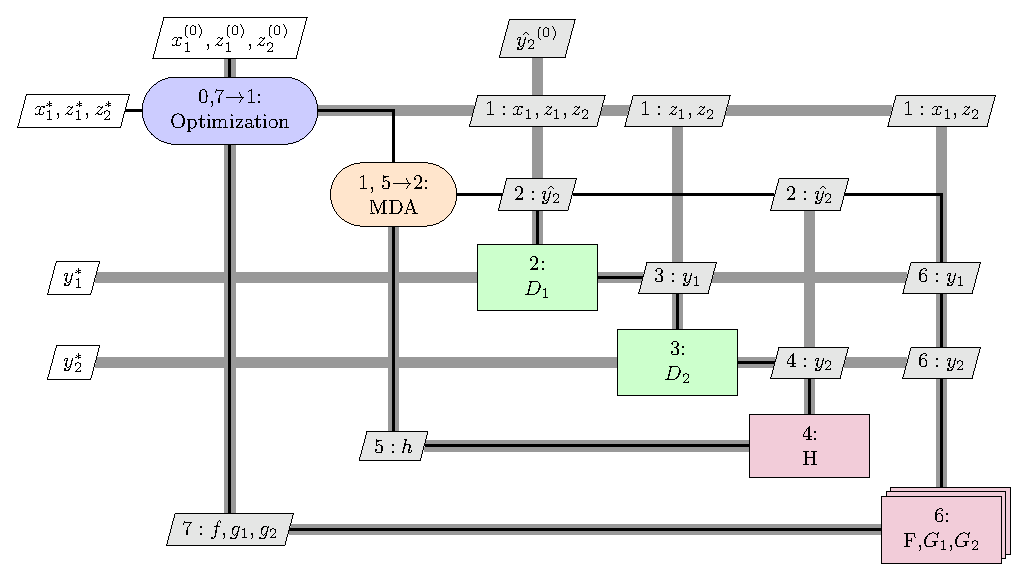
\includegraphics[height=.25\textheight]{XDSM/simple}
        \caption{XDSM for Eq. \ref{eqn:simple}, with a gauss-siedel iteration and MDF solution architecture. \label{fig:XDSM_simple}}
        \end{center}
    \end{figure}

    Although XDSM captures part of the functional aspects of FDT, it leaves out the variables themselves.  
    As a result, all variable information is aggregated 
    so that for the problem from Eq. \ref{eqn:simple_fpf} you can say that $A$ 
    depends on $B$ or vice versa, but you can't identify which 
    individual variables are interacting in the dependency cycle. 
    Without the detailed variable information, you can't construct the compatibility 
    constraints necessary to implement the problem. Additionally, XDSM 
    requires the use of solver and optimizer blocks to represent 
    the relationship between design variables and objectives/constraints. 
    By introducing solver or optimizer blocks XDSM automatically provides
    some kind of solution strategy. The XDSM for Eq. \ref{eqn:simple} is 
    given in Figure \ref{fig:XDSM_simple}. This diagram is shown with an 
    assumed gauss-siedel iteration scheme and a MDF solution architecture. 
    Hence XDSM is too specific for use with a fundamental problem formulation. 

    Of the three methods, XDSM comes the closest to fully describing a problem formulation. 
    Thought it does not contain specific variable information, this could be easily added back in
    simply by putting the variables back into the graph and drawing the apprpriat connections
    between them and the relevant analysis nodes. However, it's dependence on 
    solution strategy specifics to represent couplings can not be removed without 
    stripping it of the useful information contained in an FDT. In the following sections
    we describe a new graph syntax that retains the features of XDSM, without the dependence on 
    solution strategy (although it does allow for that information to be present). This 
    new syntax allows for the compelete specification of an FPF. 